\section{Contemporary Systems and a Comparative Case Study (2026)}
\label{sec:2026}

This survey's chronological account reaches its final year, 2026, with the two systems this paper
also uses as a focused case study. Ten further studies, taken together, show how mature the field's
evaluation culture had become by the time this survey was written.

\subsection{Ren et al.\ and Legalyze: a comparative case study}

\citet{ren2026} and Legalyze \citep{hamza2026} both appeared in 2026, and both address legal RAG,
but they target different parts of the pipeline this survey has traced since
Section~\ref{sec:rag2024}. \citet{ren2026} concentrate on the training side. They synthesize
practice-question data from source law, then use that synthetic data together with RAG, an
LLM-based judge, and an Elo-ranking mechanism to improve a legal LLM's own generation. They evaluate
it on LawBench, a benchmark for Chinese legal language models. Legalyze \citep{hamza2026} instead
concentrates on the evidence side. It preserves statutory and judicial hierarchy through
structure-aware indexing, building directly on the structure-aware indexing described in
Section~\ref{sec:rag2024}. It combines lexical and dense retrieval through reciprocal-rank fusion,
the same technique \citet{cormack2009} introduced outside the legal domain in 2009. An agentic layer
then produces a citation-grounded answer over Pakistani legal materials, extending the
jurisdiction-specific work of \citet{ref312025} from the previous year. Figure~\ref{fig:legalyze-ren}
summarizes this contrast across research objective, dataset and jurisdiction, system architecture,
core contribution, and experimental evaluation.

\begin{figure*}[tp]
\centering
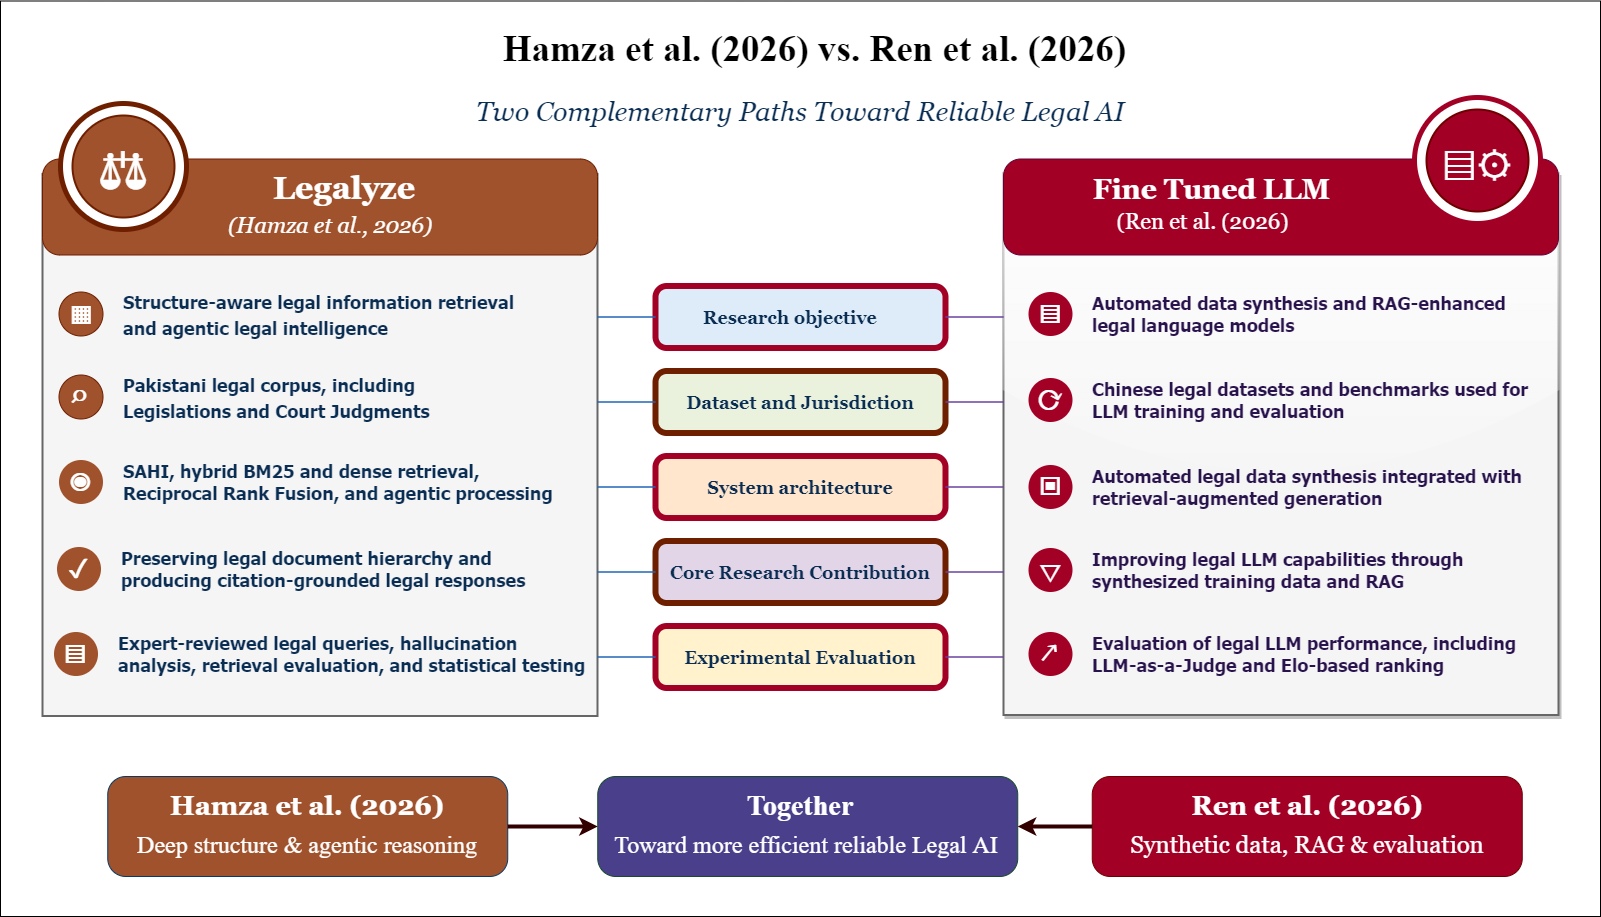
\includegraphics[width=\textwidth]{images/legalyze_vs_ren_2026_comparison.png}
\caption{Legalyze \citep{hamza2026} and the data-synthesis approach of \citet{ren2026} compared
across research objective, dataset and jurisdiction, system architecture, core research
contribution, and experimental evaluation. The two systems target different stages of the legal RAG
pipeline (evidence grounding versus training-data synthesis) and are best read as complementary
rather than directly competing.}
\label{fig:legalyze-ren}
\end{figure*}

The two approaches are complementary rather than competing. Data synthesis for training and
structure-aware retrieval for evidence grounding address different failure modes. A meaningful
head-to-head comparison would need a shared evaluation dataset, consistent query sets, and common
retrieval budgets, and none of these currently exist. Figure~\ref{fig:ren2026-arch} shows
\citeauthor{ren2026}'s own framework diagram, which makes this training-data-centric design
concrete. Data synthesis and Elo-ranking feed both a fine-tuned retrieval model and a
QLoRA-fine-tuned generation model, and together these form the Legal LLM Framework that answers a
user's query.

% Figure reproduced from Ren et al. (2026), "Automated data synthesis and
% retrieval-augmented generation for legal large language models" (Knowledge-Based
% Systems), Fig. 2, for scholarly discussion and critique within this review. Copyright
% remains with the original authors/publisher.
\begin{figure*}[t]
\centering
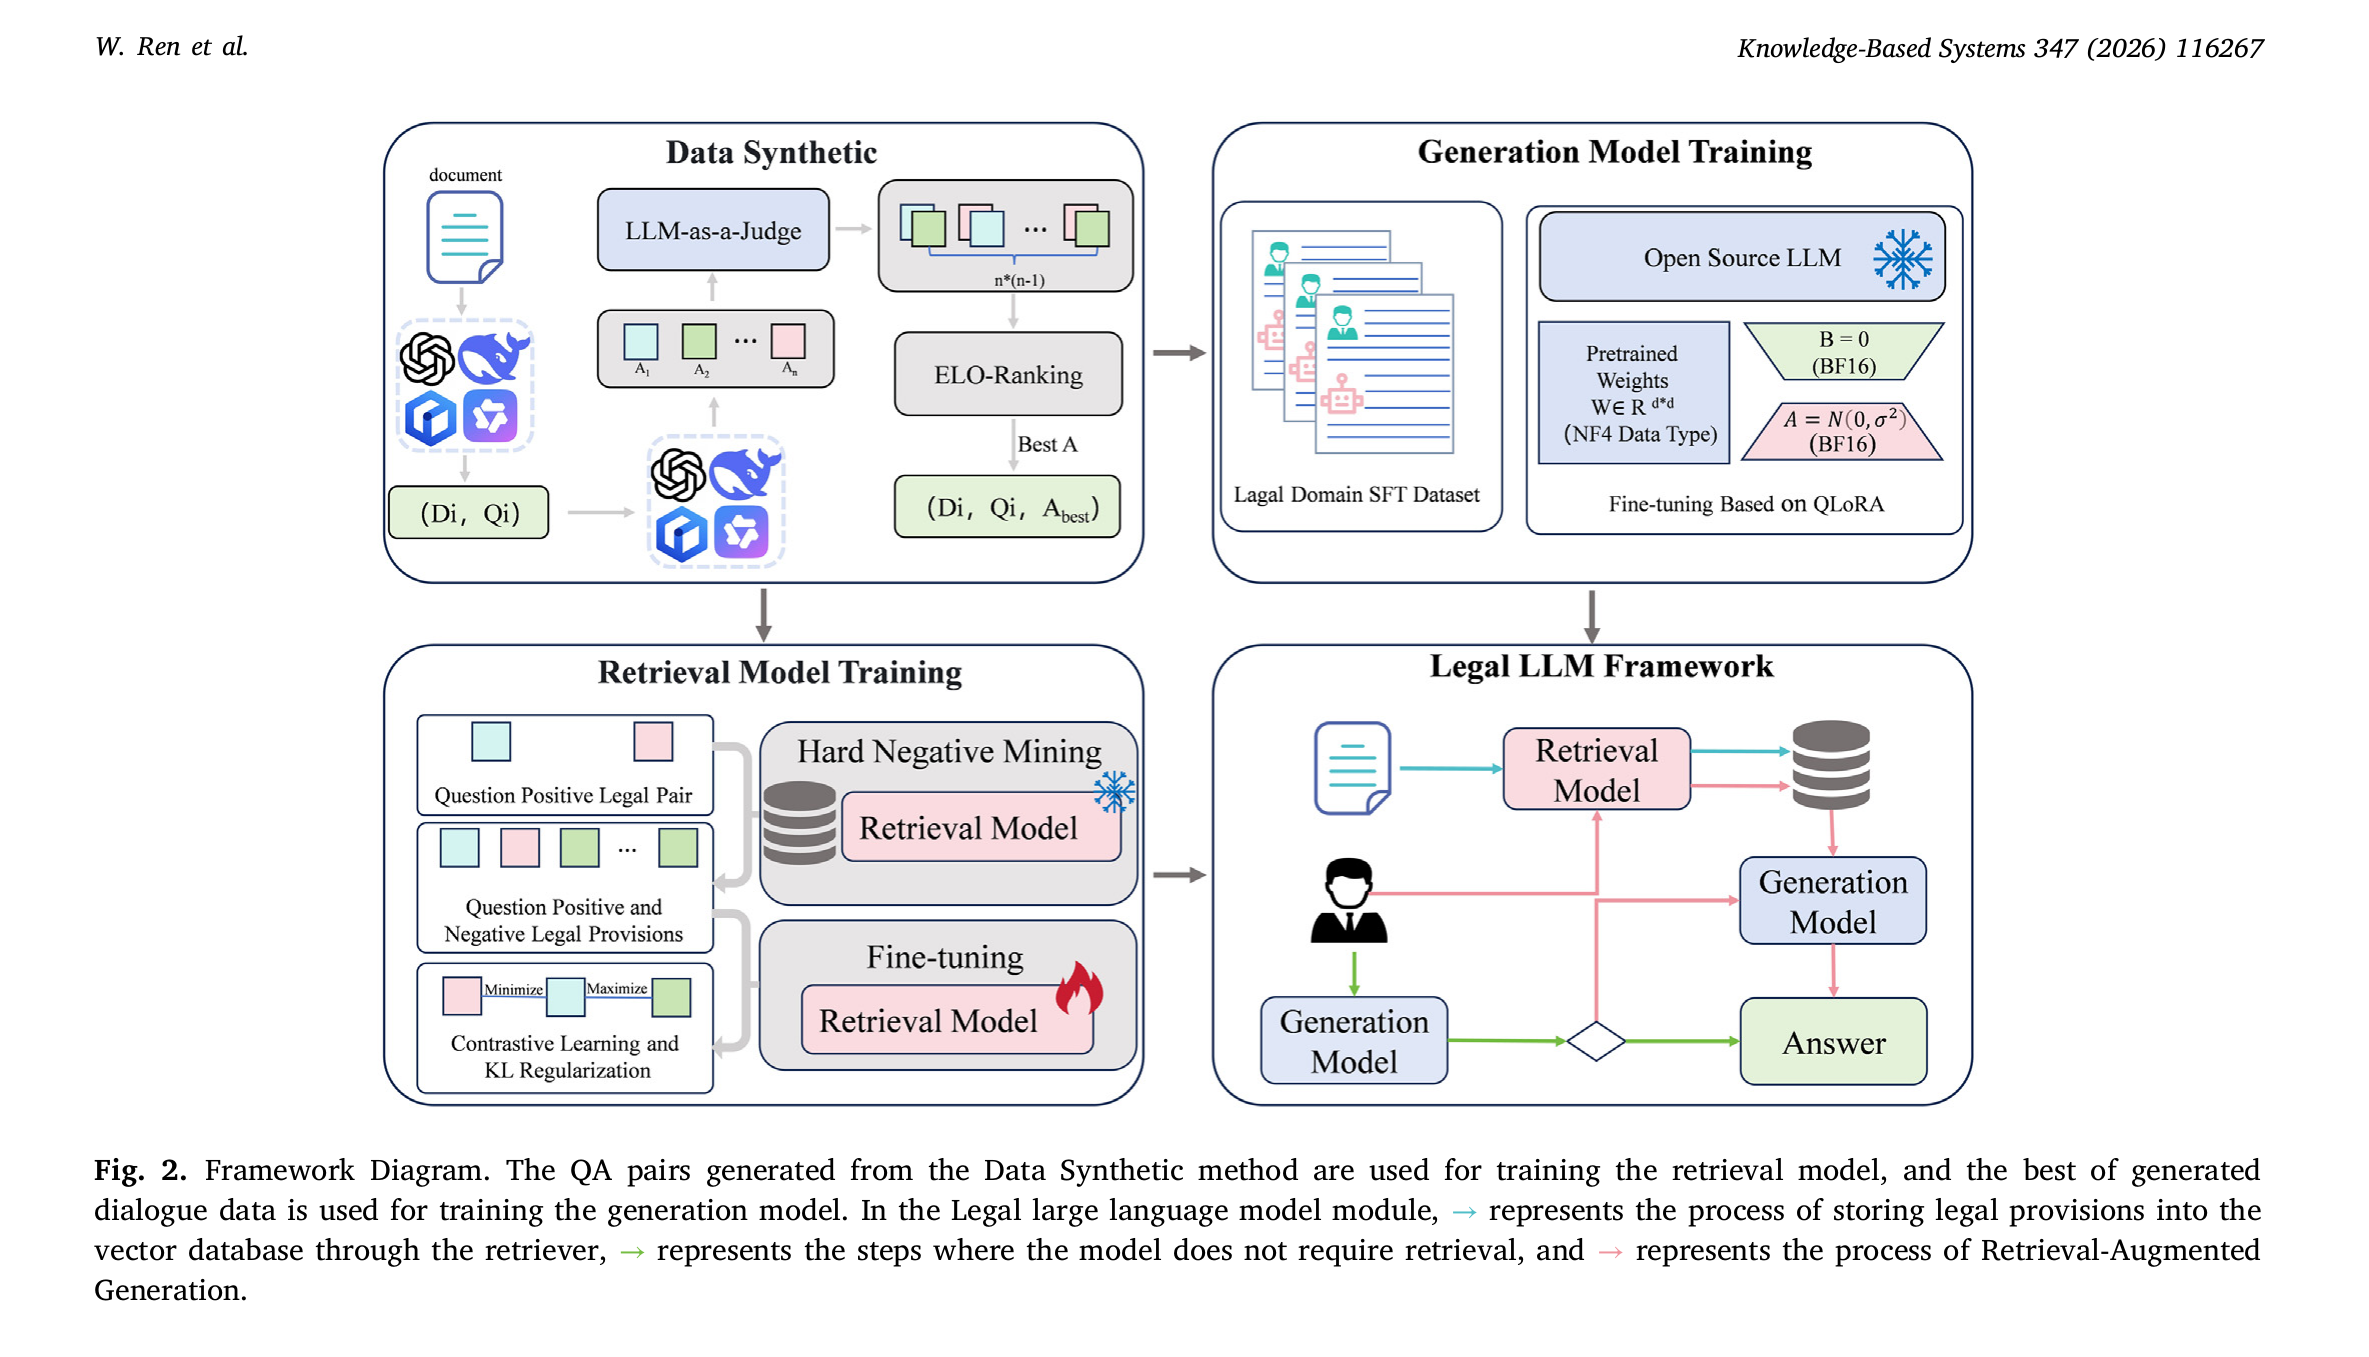
\includegraphics[width=\textwidth]{images/ren2026_fig2.png}
\caption{Figure reproduced from \citet{ren2026}: their framework diagram. QA pairs generated by
the Data Synthetic module (LLM-as-a-Judge selecting the best candidate answer via Elo-ranking)
train both the retrieval model, through hard-negative mining and contrastive fine-tuning, and the
generation model, through QLoRA fine-tuning of an open-source LLM on a legal-domain SFT dataset.
The resulting Legal LLM Framework routes a user's query through the fine-tuned retrieval model
and generation model to produce an answer, illustrating the training-data-centric design this
survey contrasts with Legalyze's evidence-centric design in Figure~\ref{fig:legalyze-ren}.}
\label{fig:ren2026-arch}
\end{figure*}


Table~\ref{tab:comp} places this pair alongside the other systems this survey has introduced
chronologically, now gathered in one place for direct comparison.

\begin{table*}[tp]
\centering
\caption{Comparison of representative legal AI systems discussed in this survey, in order of first appearance.}
\label{tab:comp}
\footnotesize
\setlength{\tabcolsep}{5pt}
\renewcommand{\arraystretch}{1.25}
\begin{tabularx}{\textwidth}{>{\raggedright\arraybackslash}p{2.6cm} >{\raggedright\arraybackslash}X >{\raggedright\arraybackslash}X >{\raggedright\arraybackslash}X}
\toprule
\textbf{System} & \textbf{Architecture and retrieval} & \textbf{Evidence verification} & \textbf{Key limitation} \\
\midrule
LEGAL-BERT \citep{chalkidis2020} & Legal-domain pretrained transformer; not inherently retrieval-based. & No inherent citation-verification mechanism. & Legal language competence does not establish evidence-grounded reasoning. \\
LexGLUE / LegalBench \citep{chalkidis2022, guha2023} & Standardized legal language and reasoning benchmarks. & Depends on the evaluated task and model. & Task scores do not directly measure citation support. \\
LegalBench-RAG \citep{pipitone2024} & Retrieval benchmark with annotated legal text segments. & Evaluates retrieval against annotated passages. & Does not, by itself, establish correctness of a generated answer. \\
JusBuild \citep{buffa2025} & Document segmentation with section-level vector retrieval for drafting. & Structured drafting workflow with human oversight. & Human review and drafting performance do not generalize to broader legal reliability. \\
Pakistani legal RAG \citep{ref312025} & Hybrid keyword and semantic retrieval over Pakistani statutes. & Grounded answering; verification assessed separately. & Grounding alone does not establish source completeness or claim-level entailment. \\
Ren et al.\ \citep{ren2026} & Synthetic data generation plus RAG for legal LLM training. & Supports the broader legal LLM pipeline. & Results depend on the selected benchmark (LawBench) and settings. \\
Legalyze \citep{hamza2026} & Hierarchical indexing, lexical and dense retrieval, reciprocal-rank fusion, agentic synthesis. & Citation-grounded response design over a hybrid retrieval pipeline. & Performance on one corpus and query set cannot establish universal correctness. \\
\bottomrule
\end{tabularx}
\end{table*}

The systems in Table~\ref{tab:comp} illustrate three design philosophies that emerged, in sequence,
across this survey's chronology. \textbf{Model-centric} approaches, LEGAL-BERT, LexGLUE, LegalBench,
adapt language models to legal text and reasoning patterns. \textbf{Retrieval-centric} approaches,
LegalBench-RAG and the Pakistani legal RAG framework, focus on locating relevant material.
\textbf{Structure-aware and workflow-oriented} approaches, JusBuild and Legalyze, also preserve
document organization. No single family addresses every legal AI problem, and evidence verification
remains distinct from retrieval in all three. That is exactly the problem
Section~\ref{sec:reliability} takes up as this survey's first synthesis chapter.

\subsection{Contemporary benchmarks, retrieval, and reasoning research}

Eight further studies from 2026 round out this survey's chronological account, each extending a
thread this survey has already introduced. \citet{yang2026} published a further survey of legal
case retrieval, extending the systematic account \citet{feng2024} gave in
Section~\ref{sec:rag2024} with two additional years of methods. \citet{goebel2026} summarized the
2025 edition of the COLIEE competition, continuing the series this survey has tracked since
\citet{goebel2023} and \citet{goebel2024}. \citet{butler2026} introduced \textbf{Legal RAG Bench},
the first full factorial evaluation of legal RAG that varies embedding models and generator LLMs
independently. They also proposed a hierarchical error-decomposition taxonomy that separates
hallucination, retrieval error, and reasoning error as distinct failure modes rather than folding
them into a single accuracy score. This taxonomy is central to how this survey discusses
reliability, so Figure~\ref{fig:rag-errors} in Section~\ref{sec:reliability} presents it in full.
\citet{chi2026} organized contemporary legal AI research around data, modelling, and evaluation,
and this survey's own methodology, in Section~\ref{sec:method}, used that broad landscape as
context for a narrower, chronological account. \citet{zhao2026} carried out a systematic review of
AI applications in litigation specifically, looking at challenges distinct from the
document-retrieval and drafting focus of most systems discussed so far. \citet{afane2026}
benchmarked legal RAG specifically on statutory surveys, testing the promise and limits of
AI-generated summaries of legislative text across jurisdictions. \citet{silva2026} evaluated RAG
systems in Brazilian civil procedure and reported a finding that echoes a theme recurring throughout
this survey since Section~\ref{sec:rag2024}: semantic similarity is not legal correctness, and a
retrieved passage that resembles the query in meaning can still fail to establish the legal point at
issue. Finally, \citet{le2026} proposed a three-tier knowledge-graph RAG architecture for legal
question answering, extending the graph-based retrieval line of work this survey has followed from
\citet{sovrano2020} in 2020, through \citet{zhu2022} in 2022, into a retrieval architecture with
three explicit levels of graph abstraction.

The chronological account is now complete, running from \citet{ashley1991} in 1991 to this final
group of 2026 studies. The rest of this survey turns from narrating the field's history to
synthesizing what it has established. Section~\ref{sec:reliability} draws together everything this
survey has said about hallucination, citation verification, and the Legal RAG Bench taxonomy just
introduced. Section~\ref{sec:jurisdiction} draws together its jurisdiction- and language-specific
findings. Section~\ref{sec:future} sets out the research agenda that follows from the complete
chronology.
